% Don't touch this %%%%%%%%%%%%%%%%%%%%%%%%%%%%%%%%%%%%%%%%%%%
\documentclass[11pt]{article}
\usepackage{fullpage}
\usepackage[left=1in,top=1in,right=1in,bottom=1in,headheight=3ex,headsep=3ex]{geometry}
\usepackage{graphicx}
\usepackage{float}
\usepackage{xcolor}
\usepackage{tikz}
\usetikzlibrary{tikzmark}
\usetikzlibrary{matrix}
\usepackage{amsmath}

\tikzset{ 
table/.style={
  matrix of nodes,
  row sep=-\pgflinewidth,
  column sep=-\pgflinewidth,
  nodes={rectangle,text width=3em,align=center},
  text depth=1.25ex,
  text height=2.5ex,
  nodes in empty cells
},
%row 1/.style={nodes={fill=green!10,text depth=0.4ex,text height=2ex}},
%row 6/.style={nodes={text depth=0.4ex,text height=2ex}},
%column 1/.style={nodes={fill=green!10}},
}

\newcommand{\blankline}{\quad\pagebreak[2]}
%%%%%%%%%%%%%%%%%%%%%%%%%%%%%%%%%%%%%%%%%%%%%%%%%%%%%%%%%%%%%%

% Modify Course title, instructor name, semester here %%%%%%%%

\title{COMP 5970/6970-004 \\ Computational Biology: Genomics and Transcriptomics \\ Lecture notes 6: 2/1/2022 }
\author{Haynes Heaton}
\date{Spring, 2022}

%%%%%%%%%%%%%%%%%%%%%%%%%%%%%%%%%%%%%%%%%%%%%%%%%%%%%%%%%%%%%%

% Don't touch this %%%%%%%%%%%%%%%%%%%%%%%%%%%%%%%%%%%%%%%%%%%
\usepackage[sc]{mathpazo}
\linespread{1.05} % Palatino needs more leading (space between lines)
%\usepackage[T1]{fontenc}
\usepackage[mmddyyyy]{datetime}% http://ctan.org/pkg/datetime
\usepackage{advdate}% http://ctan.org/pkg/advdate
\newdateformat{syldate}{\twodigit{\THEMONTH}/\twodigit{\THEDAY}}
\newsavebox{\MONDAY}\savebox{\MONDAY}{Mon}% Mon
\newcommand{\week}[1]{%
%  \cleardate{mydate}% Clear date
% \newdate{mydate}{\the\day}{\the\month}{\the\year}% Store date
  \paragraph*{\kern-2ex\quad #1, \syldate{\today} - \AdvanceDate[4]\syldate{\today}:}% Set heading  \quad #1
%  \setbox1=\hbox{\shortdayofweekname{\getdateday{mydate}}{\getdatemonth{mydate}}{\getdateyear{mydate}}}%
  \ifdim\wd1=\wd\MONDAY
    \AdvanceDate[7]
  \else
    \AdvanceDate[7]
  \fi%
}
\usepackage{setspace}
\usepackage{multicol}
%\usepackage{indentfirst}
\usepackage{fancyhdr,lastpage}
\usepackage{url}
\pagestyle{fancy}
\usepackage{hyperref}
\usepackage{lastpage}
\usepackage{amsmath}
\usepackage{layout}
\usepackage{courier}

\lhead{}
\chead{}
%%%%%%%%%%%%%%%%%%%%%%%%%%%%%%%%%%%%%%%%%%%%%%%%%%%%%%%%%%%%%%

% Modify header here %%%%%%%%%%%%%%%%%%%%%%%%%%%%%%%%%%%%%%%%%
%\rhead{\footnotesize Text in header}

%%%%%%%%%%%%%%%%%%%%%%%%%%%%%%%%%%%%%%%%%%%%%%%%%%%%%%%%%%%%%%
% Don't touch this %%%%%%%%%%%%%%%%%%%%%%%%%%%%%%%%%%%%%%%%%%%
\lfoot{}
\cfoot{\small \thepage/\pageref*{LastPage}}
\rfoot{}

\usepackage{array, xcolor}
\usepackage{color,hyperref}
\definecolor{clemsonorange}{HTML}{EA6A20}
\hypersetup{colorlinks,breaklinks,linkcolor=clemsonorange,urlcolor=clemsonorange,anchorcolor=clemsonorange,citecolor=black}

\begin{document}

\maketitle

\blankline

\begin{tabular*}{.93\textwidth}{@{\extracolsep{\fill}}lr}

%%%%%%%%%%%%%%%%%%%%%%%%%%%%%%%%%%%%%%%%%%%%%%%%%%%%%%%%%%%%%%

% Modify information %%%%%%%%%%%%%%%%%%%%%%%%%%%%%%%%%%%%%%%%%

\hline
\end{tabular*}

\vspace{5 mm}

% First Section %%%%%%%%%%%%%%%%%%%%%%%%%%%%%%%%%%%%%%%%%%%%

\section*{Lecture Objectives}
\begin{itemize}
\item Estimating statistical model parameters
\begin{itemize}
\item Maximum Likelihood methods
\begin{itemize}
\item Expectation Maximization (EM)
\item Gradient descent
\end{itemize}
\item Posterior distribution of parameters
\begin{itemize}
\item Variational Inference 
\item Markov Chain Monte Carlo (MCMC)
\end{itemize}
\end{itemize}
\item Homework 1 extra credit solution
\item Semi-Global Alignment
\item Local Alignment
\end{itemize}

\section*{Estimating statistical model parameters}
When the generation of data is not trivial, we still may be able to model it with some compound distribution or mixture of distributions. If we do not know the parameters of these distributions, they may be estimated via statistical inference. 
\subsection{Maximum Likelihood Estimation (MLE}
Last class, we did just this on a binomial mixture model with expectation maximization by starting with random model parameters and iteratively finding the posterior probability of each data point to each distribution and then updating the parameters of those distributions to improve the total likelihood. This method only guarantees finding a local optima of likelihood given a set of parameters. In certain models, this will always be the global optimum, but not all. One way to get around this is to restart the algorithm with different random parameter initializations and choosing the parameter set in which the likelihood was maximal. If the likelihood function is differentiable, another method available is gradient descent, which may be used to minimize the negative log likelihood thus maximizing the likelihood. This is also only guarantees finding a local optimum given a random initialization. In addition to this lack of global guarantee, we only find the single most likely set of parameters and do not model our uncertainty in those parameters.

\subsection{Posterior distribution of parameters}
There are a number of methods to try to model the uncertainty in the parameters as well as attempting to overcome local maxima in our likelihood landscape. Variational Inference is a method that minimizes the Kullback Leibler divergence between the data and the model distribution giving a distribution on each model parameter. However, this method also has limitations in that it also does not find a global maximum in the likelihood (or the full posterior distribution of parameters) and can only give smooth distributions over model parameters. Markov Chain Monte Carlo (MCMC) uses a probabilistic stochastic search process that, with infinite iterations, will converge to the posterior distribution. MCMC has the downside of being slow and only guaranteeing convergence to the posterior distribution with infinite iterations. I just want you all to know that these methods exist rather than knowing how they work which is out of the scope of this class. Different programming packages implement these algorithms. STAN is a domain specific language for statistical models which implements gradient descent, variational inference, and MCMC. Tensorflow probability implements gradient descent and variational inference and is a standard tool in many machine learning workflows.

\section*{Homework 1 extra credit solution}
As a reminder, the problem was  \\
7. Describe a dynamic programming approach to finding the largest checkerboard pattern in a matrix of zeros and ones where zero represents white and one represents black (checkerboard pattern is just alternating 0s and 1s, it does not matter which color starts or ends the pattern). Checkerboard must be square. Don't spend over an hour on this. If you find it difficult, come to my office hours after class and we can work through it together. Starting with 7a may help. And coming up with rules and testing them out may lead to the correct rules so use the example matrix below. \\

\noindent 7a. What is the base case for this algorithm?\\

\noindent Here is an example matrix to help develop intuition and test your method. \\

\noindent
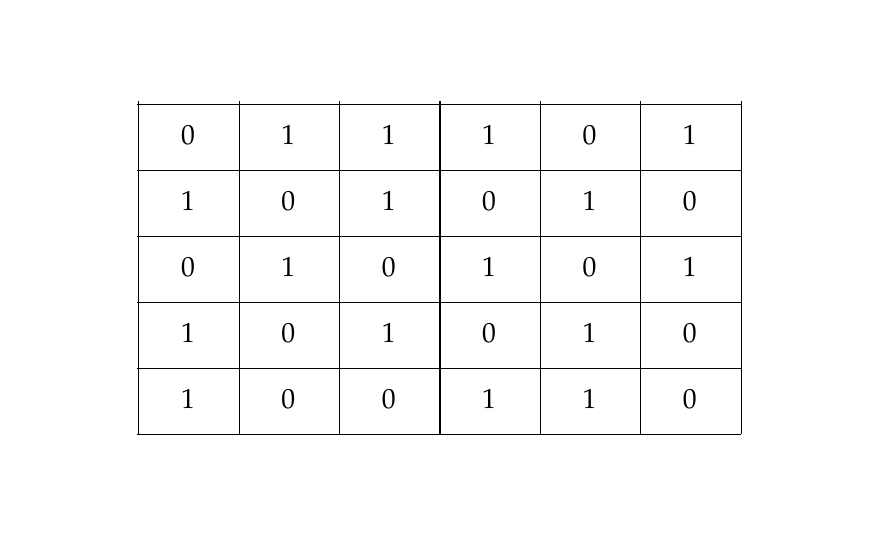
\begin{tikzpicture}
\matrix (mat) [table]
{
& & & &  &  &  & \\
& 0&1&1&1&0&1& \\
 & 1& 0& 1& 0& 1&0 &\\
 & 0& 1& 0 &1 & 0&1 &\\
 & 1& 0& 1& 0& 1 &0 &\\
 & 1& 0& 0&1 &1 & 0 &\\
 & & & & & & & \\
};
% the matrix rules
\foreach \x in {1,...,6}
{
  \draw 
    ([xshift=0\pgflinewidth]mat-\x-2.south west) --   
    ([xshift=0\pgflinewidth]mat-\x-7.south east);
  }
\foreach \x in {1,...,7}
{
  \draw 
    ([yshift=1\pgflinewidth]mat-2-\x.north east) -- 
    ([yshift=1\pgflinewidth]mat-6-\x.south east);
}    
% the arrows
\end{tikzpicture}

\noindent
Generally in dynamic programming you will have a table that keeps track of the optimal solution(s) up to this point. We need to decide what our base case solution is. In this case, the simplest base cases to use would be a $0x0$ size checkerboard or a $1x1$ checkerboard. For this example, I will use $1x1$. So a single cell of $1$ or $0$ are both $1x1$ checkerboards. Now we need to decide what the values in the DP table represent. Similar to our global alignment problem, we could have a DP table of the same size as the input matrix. In the global alignment problem, the value was the score of the alignment up until now. Here it is natural to make the DP table keep track of the largest checkerboard cell $i,j$ is the bottom right corner of. If that is the case, the left column and top row are all the base case of a $1x1$ checkerboard. We will denote the input matrix $I$ and the DP table $S$ for score. So the DP table $S$ is initialized as
\noindent
\begin{tikzpicture}
\matrix (mat) [table]
{
& & & &  &  &  & \\
& 1&1&1&1&1&1& \\
 & 1& & & & & &\\
 & 1& &  & & & &\\
 & 1& & & &  & &\\
 & 1& & & & &  &\\
 & & & & & & & \\
};
% the matrix rules
\foreach \x in {1,...,6}
{
  \draw 
    ([xshift=0\pgflinewidth]mat-\x-2.south west) --   
    ([xshift=0\pgflinewidth]mat-\x-7.south east);
  }
\foreach \x in {1,...,7}
{
  \draw 
    ([yshift=1\pgflinewidth]mat-2-\x.north east) -- 
    ([yshift=1\pgflinewidth]mat-6-\x.south east);
}    
% the arrows
\end{tikzpicture}

\noindent
Now at each $i=1..n$ and $j=1..m$, we can check the cell above and to the left of it in the input matrix and make sure they are different and the one diagonal to the upper left and make sure they are they same. If that is the case, this square is the bottom right of a checkerboard that is $min(S[i-1][j-1], S[i][j-1], S[i-1][j]) + 1$. If this isn't the case, this is only the base case checkerboard of $1x1$. So our formal recurrence relation is
\begin{equation*}
S[i,j] = 
\begin{cases}
      min(S[i-1,j-1], S[i-1][j], S[i][j-1]) + 1\\ 
      \text{\,\,\,\,\,\,\,\,\,\,\,\,if\,\,} I[i][j] = I[i-1][j-1]  \\
      \text{\,\,\,\,\,\,\,\,\,\,\,\,\,\,\,\,\,\,\,and\,\,} I[i][j] \neq I[i-1][j] \\
      \text{\,\,\,\,\,\,\,\,\,\,\,\,\,\,\,\,\,\,\,and\,\,} I[i][j] \neq I[i][j-1] \text{\,\,\,(continuation of a checkerboard)} \\
      1 \text{\,\,\,otherwise} \\
\end{cases}
\end{equation*}
So filling the DP table out, we have 

\noindent
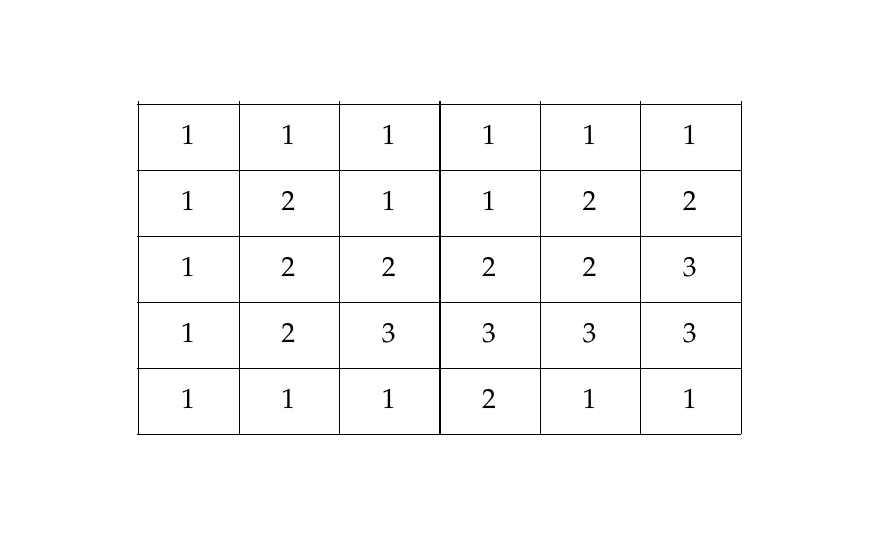
\begin{tikzpicture}
\matrix (mat) [table]
{
& & & &  &  &  & \\
& 1&1&1&1&1&1& \\
 & 1&2 & 1& 1& 2&2 &\\
 & 1& 2& 2 & 2& 2& 3&\\
 & 1& 2&3 & 3&  3&3 &\\
 & 1&1 & 1& 2& 1& 1 &\\
 & & & & & & & \\
};
% the matrix rules
\foreach \x in {1,...,6}
{
  \draw 
    ([xshift=0\pgflinewidth]mat-\x-2.south west) --   
    ([xshift=0\pgflinewidth]mat-\x-7.south east);
  }
\foreach \x in {1,...,7}
{
  \draw 
    ([yshift=1\pgflinewidth]mat-2-\x.north east) -- 
    ([yshift=1\pgflinewidth]mat-6-\x.south east);
}    
% the arrows
\end{tikzpicture} \\
\noindent
So we have several ties for different locations of a $3x3$ checkerboard in the given input matrix.

\section{Semi-Global Alignment}
\noindent
Recall our global alignment algorithm from lecture 1. One downside of this algorithm is that it assumes there is full overlap between two sequences such as shown below. \\

\begin{tikzpicture}[scale=0.75]
\draw[-] (0,0) -- (4,0);
\draw[-] (0,0.4) -- (4,0.4);
%\draw[-] (0.25,0.15) -- (0.25,0.85);
%\draw[-] (0.5,0.15) -- (0.5,0.85);
%\draw[-] (0.75,0.15) -- (0.75,0.85);
%\draw[-] (1,0.15) -- (1,0.85);
%\draw[-] (1.25,0.15) -- (1.25,0.85);
%\draw[-] (1.5,0.15) -- (1.5,0.85);
%\draw[-] (1.75,0.15) -- (1.75,0.85);
%\draw[-] (2,0.15) -- (2,0.85);
%\draw[-] (2.25,0.15) -- (2.25,0.85);
%\draw[-] (2.5,0.15) -- (2.5,0.85);
%\draw[-] (2.75,0.15) -- (2.75,0.85);
%\draw[-] (3,0.15) -- (3,0.85);
%\draw[-] (3.25,0.15) -- (3.25,0.85);
%\draw[-] (3.5,0.15) -- (3.5,0.85);
%\draw[-] (3.75,0.15) -- (3.75,0.85);
\end{tikzpicture} \\

But it is very common to want to compare two sequences which do not fully overlap. Perhaps one sequence is fully encompassed by another sequence. Or perhaps the two sequences overlap in their sequence but have overhanging ends. \\

\begin{tikzpicture}[scale=0.75]
\draw[-] (0,0.4) -- (7,0.4);
\draw[-] (2,0) -- (5,0);
%\draw[-] (2.25,0.15) -- (2.25,0.85);
%\draw[-] (2.5,0.15) -- (2.5,0.85);
%\draw[-] (2.75,0.15) -- (2.75,0.85);
%\draw[-] (3,0.15) -- (3,0.85);
%\draw[-] (3.25,0.15) -- (3.25,0.85);
%\draw[-] (3.5,0.15) -- (3.5,0.85);
%\draw[-] (3.75,0.15) -- (3.75,0.85);
%\draw[-] (4,0.15) -- (4,0.85);
%\draw[-] (4.25,0.15) -- (4.25,0.85);
%\draw[-] (4.5,0.15) -- (4.5,0.85);
%\draw[-] (4.75,0.15) -- (4.75,0.85);
\node at (9,0.5) {or};
\draw[-] (11,0.4) -- (15,0.4);
\draw[-] (12.5,0) -- (16.5,0);
%\draw[-] (12.75,0.15) -- (12.75,0.85);
%\draw[-] (13,0.15) -- (13,0.85);
%\draw[-] (13.25,0.15) -- (13.25,0.85);
%\draw[-] (13.5,0.15) -- (13.5,0.85);
%\draw[-] (13.75,0.15) -- (13.75,0.85);
%\draw[-] (14,0.15) -- (14,0.85);
%\draw[-] (14.25,0.15) -- (14.25,0.85);
%\draw[-] (14.5,0.15) -- (14.5,0.85);
%\draw[-] (14.75,0.15) -- (14.75,0.85);
\end{tikzpicture} \\

\noindent
This is known formally as semi-global alignment and informally as overlap alignment. This requires just two differences from our global alignment algorithm.
\begin{enumerate}
\item Where the Viterbi backtrace can begin and end changes from bottom right to top left to the maximum value on the bottom row or right column and goes until it hits the left column or top row.
\item The initialization of the top row and left column become all 0s as instead of them indicating indels, they indicate the start of an alignment.
\end{enumerate}
Depending on how our sequences overlap, we will have a few different patterns of where the Viterbi backtrace begins and ends. \\

\begin{tikzpicture}[scale=0.75]
\draw[-] (0,0.4) -- (7,0.4);
\draw[-] (2,0) -- (5,0);
%\draw[-] (2.25,0.15) -- (2.25,0.85);
%\draw[-] (2.5,0.15) -- (2.5,0.85);
%\draw[-] (2.75,0.15) -- (2.75,0.85);
%\draw[-] (3,0.15) -- (3,0.85);
%\draw[-] (3.25,0.15) -- (3.25,0.85);
%\draw[-] (3.5,0.15) -- (3.5,0.85);
%\draw[-] (3.75,0.15) -- (3.75,0.85);
%\draw[-] (4,0.15) -- (4,0.85);
%\draw[-] (4.25,0.15) -- (4.25,0.85);
%\draw[-] (4.5,0.15) -- (4.5,0.85);
%\draw[-] (4.75,0.15) -- (4.75,0.85);
%\node at (9,0.5) {or};
\node at (3.5,0.7) {x};
\node at (3.5,-0.4) {y};
\draw[-] (0,-2) -- (7,-2);
\draw[-] (0,-2) -- (0,-5);
\draw[-] (7,-2) -- (7,-5);
\draw[-] (0,-5) -- (7,-5);
\node at (-0.3,-3.4) {y};
\node at (3.5,-1.7) {x};
\draw[-] (5,-5) -- (2, -2);

\draw[-] (11,0.4) -- (15,0.4);
\draw[-] (12.5,0) -- (16.5,0);
%\draw[-] (12.75,0.15) -- (12.75,0.85);
%\draw[-] (13,0.15) -- (13,0.85);
%\draw[-] (13.25,0.15) -- (13.25,0.85);
%\draw[-] (13.5,0.15) -- (13.5,0.85);
%\draw[-] (13.75,0.15) -- (13.75,0.85);
%\draw[-] (14,0.15) -- (14,0.85);
%\draw[-] (14.25,0.15) -- (14.25,0.85);
%\draw[-] (14.5,0.15) -- (14.5,0.85);
%\draw[-] (14.75,0.15) -- (14.75,0.85);
\node at (13,0.7) {x};
\node at (14.5,-0.4) {y};

\draw[-] (11.75,-2) -- (15.75,-2);
\draw[-] (11.75,-2) -- (11.75,-6);
\draw[-] (15.75,-2) -- (15.75,-6);
\draw[-] (11.75,-6) -- (15.75,-6);
\node at (13.75, -1.7) {x};
\node at (11.75-0.3,-4) {y};
\draw[-] (15.75-2.5,-2) -- (15.75,-2-2.5);

\end{tikzpicture} \\
and \\ \\
\begin{tikzpicture}[scale=0.75]
\draw[-] (0,0) -- (7,0);
\draw[-] (2,0.4) -- (5,0.4);
\node at (3.5,0.7) {x};
\node at (3.5,-0.4) {y};
\draw[-] (2,-2) -- (5,-2);
\draw[-] (2,-2) -- (2,-9);
\draw[-] (5,-2) -- (5,-9);
\draw[-] (2,-9) -- (5,-9);
\node at (1.7,-5.5) {y};
\node at (3.5,-1.7) {x};
\draw[-] (5,-7) -- (2, -4);

\draw[-] (11,0) -- (15,0);
\draw[-] (12.5,0.4) -- (16.5,0.4);
%\draw[-] (12.75,0.15) -- (12.75,0.85);
%\draw[-] (13,0.15) -- (13,0.85);
%\draw[-] (13.25,0.15) -- (13.25,0.85);
%\draw[-] (13.5,0.15) -- (13.5,0.85);
%\draw[-] (13.75,0.15) -- (13.75,0.85);
%\draw[-] (14,0.15) -- (14,0.85);
%\draw[-] (14.25,0.15) -- (14.25,0.85);
%\draw[-] (14.5,0.15) -- (14.5,0.85);
%\draw[-] (14.75,0.15) -- (14.75,0.85);
\node at (13,-0.4) {y};
\node at (14.5,0.7) {x};

\draw[-] (11.75,-2) -- (15.75,-2);
\draw[-] (11.75,-2) -- (11.75,-6);
\draw[-] (15.75,-2) -- (15.75,-6);
\draw[-] (11.75,-6) -- (15.75,-6);
\node at (13.75, -1.7) {x};
\node at (11.75-0.3,-4) {y};
\draw[-] (11.75,-6+2.5) -- (11.75+2.5,-6);

\end{tikzpicture} \\

\noindent So in this case, we initialize the top row and left column with 0s indicating possible starts of an overlap alignment. \\ \\
\noindent
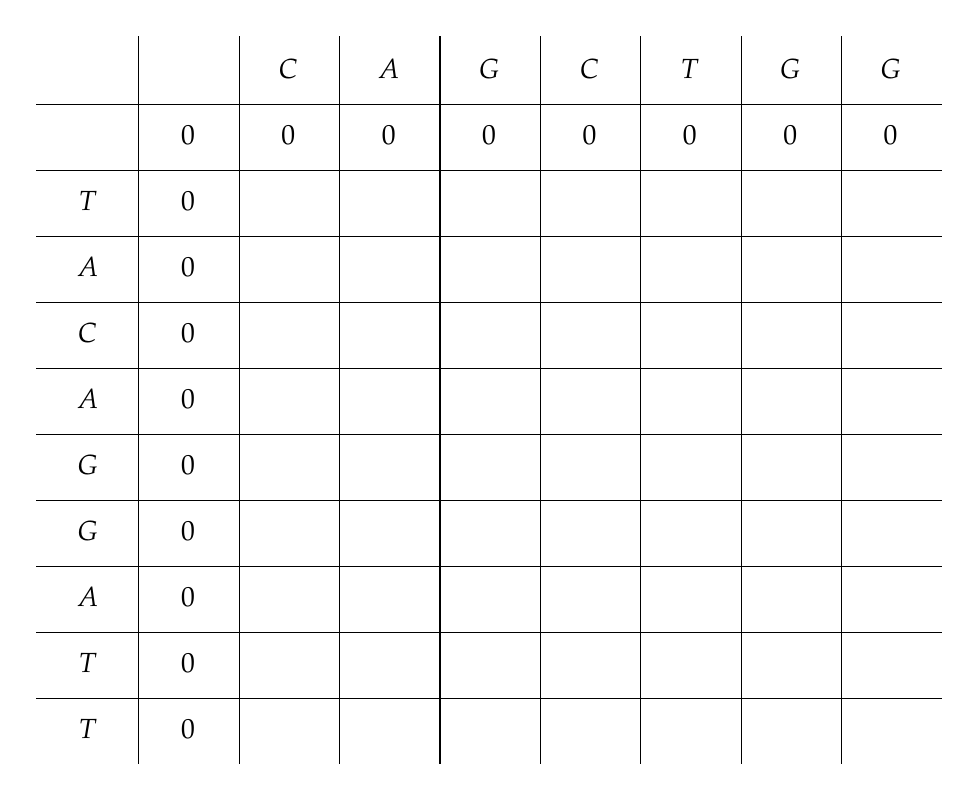
\begin{tikzpicture}[scale=0.5]
\matrix (mat) [table, scale=0.8]
{
& & $C$ & $A$ & $G$ & $C$ & $T$ & $G$ & $G$ \\
&0 &0&0&0&0&0&0&0 \\
$T$ & 0& & & & & &&\\
$A$ & 0& &  & & & &&\\
$C$ & 0& & & &  & &&\\
$A$ & 0& & & & &  &&\\
$G$ & 0& & & & & && \\
$G$ & 0& & & & & && \\
$A$ & 0& & & & & && \\
$T$ & 0& & & & & && \\
$T$ & 0& & & & & && \\
};
% the matrix rules
\foreach \x in {1,...,10}
{
  \draw 
    ([xshift=-.5\pgflinewidth]mat-\x-1.south west) --   
    ([xshift=-.5\pgflinewidth]mat-\x-9.south east);
  }
\foreach \x in {1,...,8}
{
  \draw 
    ([yshift=.5\pgflinewidth]mat-1-\x.north east) -- 
    ([yshift=.5\pgflinewidth]mat-11-\x.south east);
}    
% the arrows
\end{tikzpicture} \\

And we proceed as we did in the global alignment for filling out the score matrix. As a reminder, the recurrence relation is

\begin{equation*}
m[i,j] = max
\begin{cases}
      m[i-1,j-1] + 1 & \text{if \,\, } s_1[i] = s_2[j] \text{ (match)} \\
      m[i-1,j-1] - 1 &  \text{if \,\, } s_1[i] \neq s_2[j] \text{ (mismatch)} \\
      m[i-1,j] - 1 \text{ (indel)} \\
      m[i,j-1] - 1 \text{ (indel)} \\
\end{cases}
\end{equation*}

\noindent
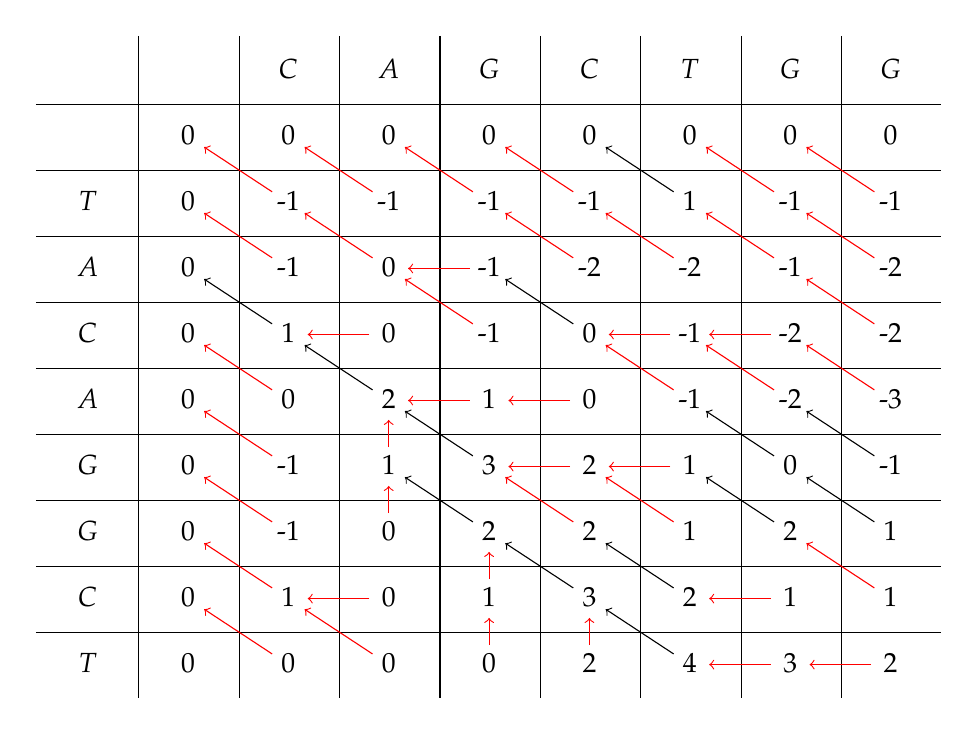
\begin{tikzpicture}[scale=0.8]
\matrix (mat) [table]
{
& & $C$ & $A$ & $G$ & $C$ & $T$ & $G$ & $G$ \\
&0 &0&0&0&0&0&0&0 \\
$T$ & 0& -1 & -1 &-1 & -1& 1 &-1 & -1 \\
$A$ & 0& -1 & 0 & -1 & -2 &-2 &-1&-2\\
$C$ & 0&1&0 &-1 &  0&-1 &-2&-2 \\
$A$ & 0& 0& 2& 1& 0& -1 &-2&-3\\
$G$ & 0&-1&1 & 3&2 &1 &0& -1\\
$G$ & 0&-1 &0 &2 & 2&1 &2&1 \\
$C$ & 0& 1& 0& 1& 3& 2&1&1 \\
$T$ & 0& 0& 0&0 &2 &4 &3&2 \\
};
% the matrix rules
\foreach \x in {1,...,9}
{
  \draw 
    ([xshift=-.5\pgflinewidth]mat-\x-1.south west) --   
    ([xshift=-.5\pgflinewidth]mat-\x-9.south east);
  }
\foreach \x in {1,...,8}
{
  \draw 
    ([yshift=.5\pgflinewidth]mat-1-\x.north east) -- 
    ([yshift=.5\pgflinewidth]mat-10-\x.south east);
}    
% the arrows
\begin{scope}[shorten >=7pt,shorten <= 7pt]
\draw[red,->]  (mat-3-3.center) -- (mat-2-2.center);
\draw[red,->]  (mat-4-3.center) -- (mat-3-2.center);
\draw[->]  (mat-5-3.center) -- (mat-4-2.center);
\draw[red,->]  (mat-6-3.center) -- (mat-5-2.center);
\draw[red,->]  (mat-7-3.center) -- (mat-6-2.center);
\draw[red,->]  (mat-8-3.center) -- (mat-7-2.center);
\draw[red,->]  (mat-9-3.center) -- (mat-8-2.center);
\draw[red,->]  (mat-10-3.center) -- (mat-9-2.center);
%\draw[red,->]  (mat-11-3.center) -- (mat-10-2.center);
\draw[red,->]  (mat-3-4.center) -- (mat-2-3.center);
\draw[red,->]  (mat-3-5.center) -- (mat-2-4.center);
\draw[red,->]  (mat-3-6.center) -- (mat-2-5.center);
\draw[->]  (mat-3-7.center) -- (mat-2-6.center);
\draw[red,->]  (mat-3-8.center) -- (mat-2-7.center);
\draw[red,->]  (mat-3-9.center) -- (mat-2-8.center);

\draw[red,->]  (mat-4-4.center) -- (mat-3-3.center);
\draw[red,->]  (mat-4-5.center) -- (mat-4-4.center);
\draw[red,->]  (mat-4-6.center) -- (mat-3-5.center);
\draw[red,->]  (mat-4-7.center) -- (mat-3-6.center);
\draw[red,->]  (mat-4-8.center) -- (mat-3-7.center);
\draw[red,->]  (mat-4-9.center) -- (mat-3-8.center);
\draw[red,->]  (mat-5-4.center) -- (mat-5-3.center);
\draw[red,->]  (mat-5-5.center) -- (mat-4-4.center);
\draw[->]  (mat-5-6.center) -- (mat-4-5.center);
\draw[red,->]  (mat-5-7.center) -- (mat-5-6.center);
\draw[red,->]  (mat-5-8.center) -- (mat-5-7.center);
\draw[red,->]  (mat-5-9.center) -- (mat-4-8.center);
\draw[->]  (mat-6-4.center) -- (mat-5-3.center);
\draw[red,->]  (mat-6-5.center) -- (mat-6-4.center);
\draw[red,->]  (mat-6-6.center) -- (mat-6-5.center);
\draw[red,->]  (mat-6-7.center) -- (mat-5-6.center);
\draw[red,->]  (mat-6-8.center) -- (mat-5-7.center);
\draw[red,->]  (mat-6-9.center) -- (mat-5-8.center);
\draw[red,->]  (mat-7-4.center) -- (mat-6-4.center);
\draw[->]  (mat-7-5.center) -- (mat-6-4.center);
\draw[red,->]  (mat-7-6.center) -- (mat-7-5.center);
\draw[red,->]  (mat-7-7.center) -- (mat-7-6.center);
\draw[->]  (mat-7-8.center) -- (mat-6-7.center);
\draw[->]  (mat-7-9.center) -- (mat-6-8.center);
\draw[red,->]  (mat-8-4.center) -- (mat-7-4.center);
\draw[->]  (mat-8-5.center) -- (mat-7-4.center);
\draw[red,->]  (mat-8-6.center) -- (mat-7-5.center);
\draw[red,->]  (mat-8-7.center) -- (mat-7-6.center);
\draw[->]  (mat-8-8.center) -- (mat-7-7.center);
\draw[->]  (mat-8-9.center) -- (mat-7-8.center);
\draw[red,->]  (mat-9-4.center) -- (mat-9-3.center);
\draw[red,->]  (mat-9-5.center) -- (mat-8-5.center);
\draw[->]  (mat-9-6.center) -- (mat-8-5.center);
\draw[->]  (mat-9-7.center) -- (mat-8-6.center);
\draw[red,->]  (mat-9-8.center) -- (mat-9-7.center);
\draw[red,->]  (mat-9-9.center) -- (mat-8-8.center);
\draw[red,->]  (mat-10-4.center) -- (mat-9-3.center);
\draw[red,->]  (mat-10-5.center) -- (mat-9-5.center);
\draw[red,->]  (mat-10-6.center) -- (mat-9-6.center);
\draw[->]  (mat-10-7.center) -- (mat-9-6.center);
\draw[red,->]  (mat-10-8.center) -- (mat-10-7.center);
\draw[red,->]  (mat-10-9.center) -- (mat-10-8.center);
\end{scope}
\end{tikzpicture} \\

Now we take the maximum value in the bottom row or right column to begin the backtrace algorithm. This is the value 4. So we have the following backtrace.


\noindent
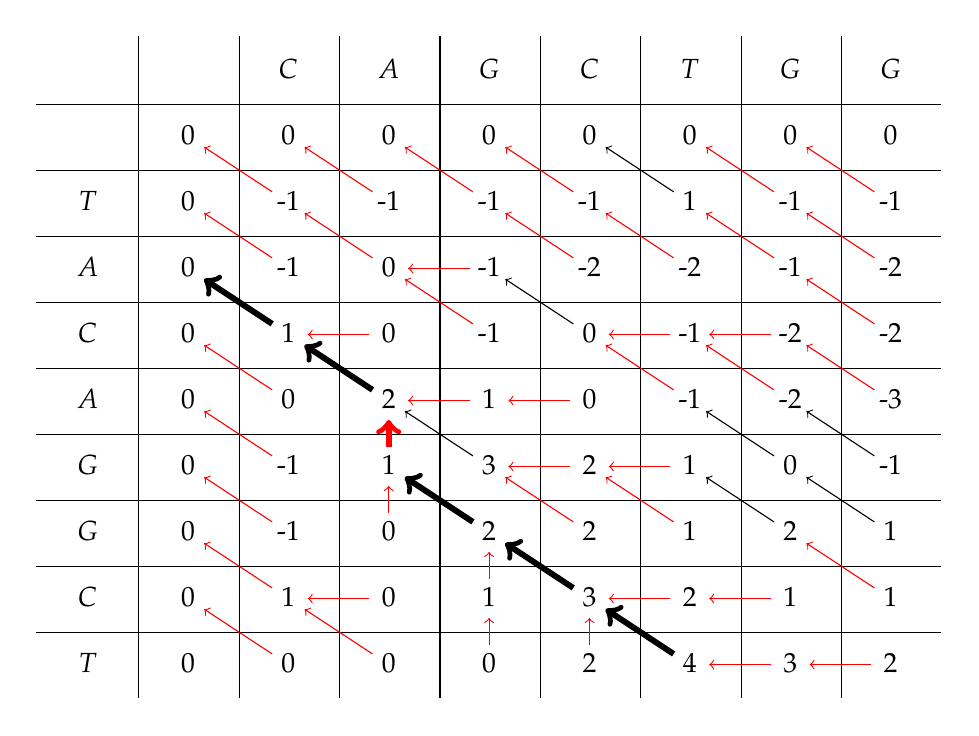
\begin{tikzpicture}[scale=0.8]
\matrix (mat) [table]
{
& & $C$ & $A$ & $G$ & $C$ & $T$ & $G$ & $G$ \\
&0 &0&0&0&0&0&0&0 \\
$T$ & 0& -1 & -1 &-1 & -1& 1 &-1 & -1 \\
$A$ & 0& -1 & 0 & -1 & -2 &-2 &-1&-2\\
$C$ & 0&1&0 &-1 &  0&-1 &-2&-2 \\
$A$ & 0& 0& 2& 1& 0& -1 &-2&-3\\
$G$ & 0&-1&1 & 3&2 &1 &0& -1\\
$G$ & 0&-1 &0 &2 & 2&1 &2&1 \\
$C$ & 0& 1& 0& 1& 3& 2&1&1 \\
$T$ & 0& 0& 0&0 &2 &4 &3&2 \\
};
% the matrix rules
\foreach \x in {1,...,9}
{
  \draw 
    ([xshift=-.5\pgflinewidth]mat-\x-1.south west) --   
    ([xshift=-.5\pgflinewidth]mat-\x-9.south east);
  }
\foreach \x in {1,...,8}
{
  \draw 
    ([yshift=.5\pgflinewidth]mat-1-\x.north east) -- 
    ([yshift=.5\pgflinewidth]mat-10-\x.south east);
}    
% the arrows
\begin{scope}[shorten >=7pt,shorten <= 7pt]
\draw[red,->]  (mat-3-3.center) -- (mat-2-2.center);
\draw[red,->]  (mat-4-3.center) -- (mat-3-2.center);
\draw[line width =.75mm,->]  (mat-5-3.center) -- (mat-4-2.center);
\draw[red,->]  (mat-6-3.center) -- (mat-5-2.center);
\draw[red,->]  (mat-7-3.center) -- (mat-6-2.center);
\draw[red,->]  (mat-8-3.center) -- (mat-7-2.center);
\draw[red,->]  (mat-9-3.center) -- (mat-8-2.center);
\draw[red,->]  (mat-10-3.center) -- (mat-9-2.center);
%\draw[red,->]  (mat-11-3.center) -- (mat-10-2.center);
\draw[red,->]  (mat-3-4.center) -- (mat-2-3.center);
\draw[red,->]  (mat-3-5.center) -- (mat-2-4.center);
\draw[red,->]  (mat-3-6.center) -- (mat-2-5.center);
\draw[->]  (mat-3-7.center) -- (mat-2-6.center);
\draw[red,->]  (mat-3-8.center) -- (mat-2-7.center);
\draw[red,->]  (mat-3-9.center) -- (mat-2-8.center);

\draw[red,->]  (mat-4-4.center) -- (mat-3-3.center);
\draw[red,->]  (mat-4-5.center) -- (mat-4-4.center);
\draw[red,->]  (mat-4-6.center) -- (mat-3-5.center);
\draw[red,->]  (mat-4-7.center) -- (mat-3-6.center);
\draw[red,->]  (mat-4-8.center) -- (mat-3-7.center);
\draw[red,->]  (mat-4-9.center) -- (mat-3-8.center);
\draw[red,->]  (mat-5-4.center) -- (mat-5-3.center);
\draw[red,->]  (mat-5-5.center) -- (mat-4-4.center);
\draw[->]  (mat-5-6.center) -- (mat-4-5.center);
\draw[red,->]  (mat-5-7.center) -- (mat-5-6.center);
\draw[red,->]  (mat-5-8.center) -- (mat-5-7.center);
\draw[red,->]  (mat-5-9.center) -- (mat-4-8.center);
\draw[line width =.75mm,->]  (mat-6-4.center) -- (mat-5-3.center);
\draw[red,->]  (mat-6-5.center) -- (mat-6-4.center);
\draw[red,->]  (mat-6-6.center) -- (mat-6-5.center);
\draw[red,->]  (mat-6-7.center) -- (mat-5-6.center);
\draw[red,->]  (mat-6-8.center) -- (mat-5-7.center);
\draw[red,->]  (mat-6-9.center) -- (mat-5-8.center);
\draw[line width =.75mm,red,->]  (mat-7-4.center) -- (mat-6-4.center);
\draw[->]  (mat-7-5.center) -- (mat-6-4.center);
\draw[red,->]  (mat-7-6.center) -- (mat-7-5.center);
\draw[red,->]  (mat-7-7.center) -- (mat-7-6.center);
\draw[->]  (mat-7-8.center) -- (mat-6-7.center);
\draw[->]  (mat-7-9.center) -- (mat-6-8.center);
\draw[red,->]  (mat-8-4.center) -- (mat-7-4.center);
\draw[line width =.75mm,->]  (mat-8-5.center) -- (mat-7-4.center);
\draw[red,->]  (mat-8-6.center) -- (mat-7-5.center);
\draw[red,->]  (mat-8-7.center) -- (mat-7-6.center);
\draw[->]  (mat-8-8.center) -- (mat-7-7.center);
\draw[->]  (mat-8-9.center) -- (mat-7-8.center);
\draw[red,->]  (mat-9-4.center) -- (mat-9-3.center);
\draw[red,->]  (mat-9-5.center) -- (mat-8-5.center);
\draw[line width =.75mm,->]  (mat-9-6.center) -- (mat-8-5.center);
\draw[red,->]  (mat-9-7.center) -- (mat-9-6.center);
\draw[red,->]  (mat-9-8.center) -- (mat-9-7.center);
\draw[red,->]  (mat-9-9.center) -- (mat-8-8.center);
\draw[red,->]  (mat-10-4.center) -- (mat-9-3.center);
\draw[red,->]  (mat-10-5.center) -- (mat-9-5.center);
\draw[red,->]  (mat-10-6.center) -- (mat-9-6.center);
\draw[line width =.75mm,->]  (mat-10-7.center) -- (mat-9-6.center);
\draw[red,->]  (mat-10-8.center) -- (mat-10-7.center);
\draw[red,->]  (mat-10-9.center) -- (mat-10-8.center);
\end{scope}
\end{tikzpicture} \\


\noindent
Creating an alignment of \\
\mbox{\texttt{ CA-GCTGG}} \\
\texttt{TCAGGCT} \\ \\

\section*{Local Alignment - AKA Smith-Waterman}


The next type of alignment is when you expect two sequences to only align in a subsequence of both sequences rather than an overlap or a full length alignment. Again, this is a small difference from the previous alignment algorithms.
\begin{enumerate}
\item Whenever an alignment score would go negative, instead it starts a new alignment with score 0
\item The Viterbi backtrace starts and the maximum score in the entire matrix and goes back to the first 0 the backtrace encounters
\end{enumerate}

\begin{equation*}
m[i,j] = max
\begin{cases}
      m[i-1,j-1] + 1 & \text{if \,\, } s_1[i] = s_2[j] \text{ (match)} \\
      m[i-1,j-1] - 1 &  \text{if \,\, } s_1[i] \neq s_2[j] \text{ (mismatch)} \\
      m[i-1,j] - 1 \text{ (indel)} \\
      m[i,j-1] - 1 \text{ (indel)} \\
      0 \text{\,\,\,(start new alignment)}\\
\end{cases}
\end{equation*}

So we once again initialize the top row and left column with alignments starting with a score of 0.

\noindent
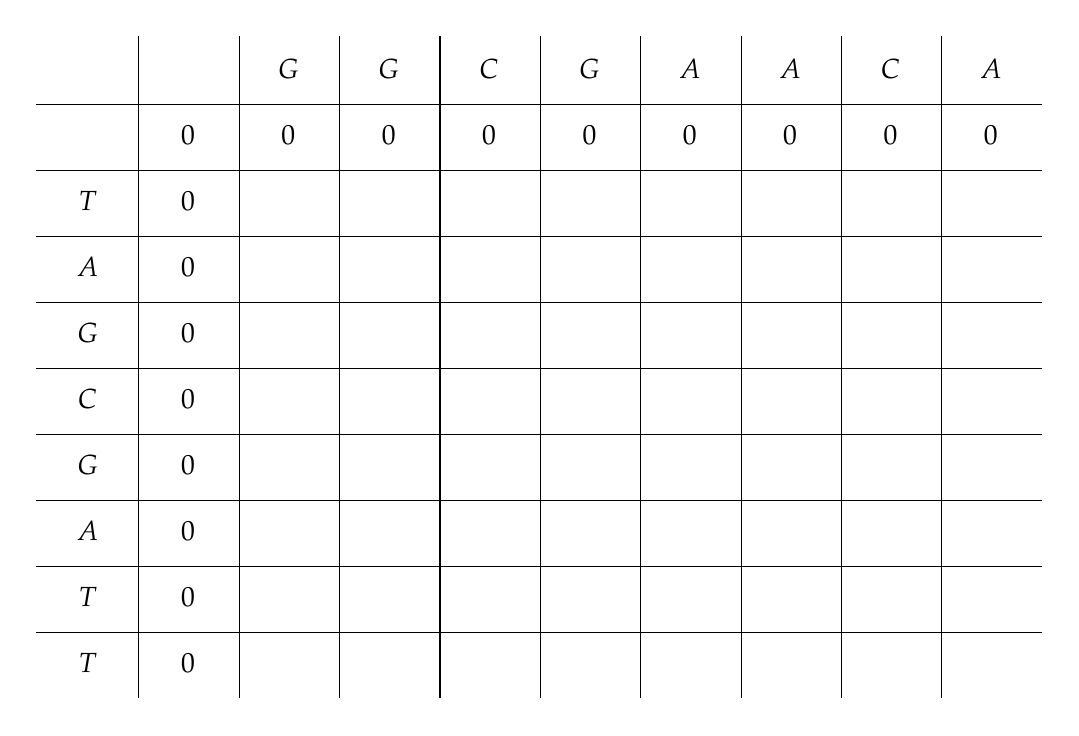
\begin{tikzpicture}[scale=0.8]
\matrix (mat) [table]
{
& & $G$ & $G$ & $C$ & $G$ & $A$ & $A$ & $C$ & $A$ \\
&0 &0&0&0&0&0&0&0 &0 \\
$T$ & 0&  &  & & &  & & & \\
$A$ & 0&  &  &  &  & &&&\\
$G$ & 0&& & &  & &&& \\
$C$ & 0& & & & &  &&&\\
$G$ & 0&&& & & &&&\\
$A$ & 0& & & & & && &\\
$T$ & 0& & & & & && &\\
$T$ & 0& & & & & &&& \\
};
% the matrix rules
\foreach \x in {1,...,9}
{
  \draw 
    ([xshift=-.5\pgflinewidth]mat-\x-1.south west) --   
    ([xshift=-.5\pgflinewidth]mat-\x-10.south east);
  }
\foreach \x in {1,...,9}
{
  \draw 
    ([yshift=.5\pgflinewidth]mat-1-\x.north east) -- 
    ([yshift=.5\pgflinewidth]mat-10-\x.south east);
}    
% the arrows
\end{tikzpicture} \\

\noindent
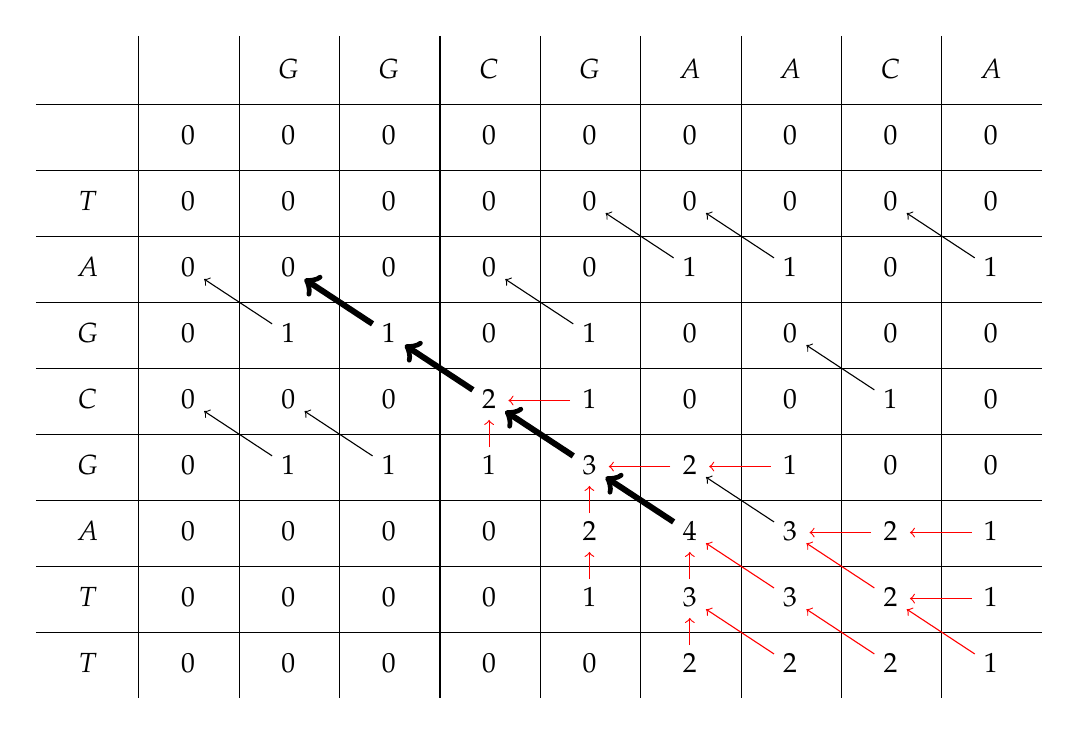
\begin{tikzpicture}[scale=0.8]
\matrix (mat) [table]
{
& & $G$ & $G$ & $C$ & $G$ & $A$ & $A$ & $C$ & $A$ \\
&0 &0&0&0&0&0&0&0 &0 \\
$T$ & 0& 0 & 0 & 0& 0& 0 & 0& 0& 0\\
$A$ & 0& 0 & 0 & 0 & 0 & 1&1&0&1\\
$G$ & 0&1&1 & 0&  1&0 &0&0&0 \\
$C$ & 0&0 &0 &2 & 1& 0 &0&1&0\\
$G$ & 0&1&1& 1&3 & 2&1&0&0\\
$A$ & 0& 0&0 &0 &2 &4 &3&2 &1\\
$T$ & 0& 0& 0& 0& 1& 3&3&2 &1\\
$T$ & 0& 0& 0&0 &0 &2 &2&2&1 \\
};
% the matrix rules
\foreach \x in {1,...,9}
{
  \draw 
    ([xshift=-.5\pgflinewidth]mat-\x-1.south west) --   
    ([xshift=-.5\pgflinewidth]mat-\x-10.south east);
  }
\foreach \x in {1,...,9}
{
  \draw 
    ([yshift=.5\pgflinewidth]mat-1-\x.north east) -- 
    ([yshift=.5\pgflinewidth]mat-10-\x.south east);
}    
% the arrows
\begin{scope}[shorten >=7pt,shorten <= 7pt]

\draw[->]  (mat-5-3.center) -- (mat-4-2.center);
\draw[->]  (mat-7-3.center) -- (mat-6-2.center);
\draw[->]  (mat-4-7.center) -- (mat-3-6.center);
\draw[->]  (mat-4-8.center) -- (mat-3-7.center);
\draw[->]  (mat-4-10.center) -- (mat-3-9.center);
\draw[line width =.75mm,->]  (mat-5-4.center) -- (mat-4-3.center);
\draw[->]  (mat-5-6.center) -- (mat-4-5.center);
\draw[line width =.75mm,->]  (mat-6-5.center) -- (mat-5-4.center);
\draw[red,->]  (mat-6-6.center) -- (mat-6-5.center);
\draw[->]  (mat-6-9.center) -- (mat-5-8.center);
\draw[->]  (mat-7-4.center) -- (mat-6-3.center);
\draw[red,->]  (mat-7-5.center) -- (mat-6-5.center);
\draw[line width =.75mm,->]  (mat-7-6.center) -- (mat-6-5.center);
\draw[red,->]  (mat-7-7.center) -- (mat-7-6.center);
\draw[red,->]  (mat-7-8.center) -- (mat-7-7.center);
\draw[red,->]  (mat-8-6.center) -- (mat-7-6.center);
\draw[line width =.75mm,->]  (mat-8-7.center) -- (mat-7-6.center);
\draw[->]  (mat-8-8.center) -- (mat-7-7.center);
\draw[red,->]  (mat-8-9.center) -- (mat-8-8.center);
\draw[red,->]  (mat-8-10.center) -- (mat-8-9.center);
\draw[red,->]  (mat-9-6.center) -- (mat-8-6.center);
\draw[red,->]  (mat-9-7.center) -- (mat-8-7.center);
\draw[red,->]  (mat-9-8.center) -- (mat-8-7.center);
\draw[red,->]  (mat-9-9.center) -- (mat-8-8.center);
\draw[red,->]  (mat-9-10.center) -- (mat-9-9.center);
\draw[red,->]  (mat-10-7.center) -- (mat-9-7.center);
\draw[red,->]  (mat-10-8.center) -- (mat-9-7.center);
\draw[red,->]  (mat-10-9.center) -- (mat-9-8.center);
\draw[red,->]  (mat-10-10.center) -- (mat-9-9.center);
\end{scope}
\end{tikzpicture} \\
\noindent
Creating an alignment of \\
\texttt{GCGA} \\
\texttt{GCGA} \\ \\
with the rest of the sequence unaligned.

\end{document}
